\section{Method}
\subsection{Problem formulation}
The PCB was tested using the National Instruments myDAQ, by powering the PCB with the myDAQ:s constant 5V output and then imposing a square wave on the input pin with following characteristics:
\begin{itemize}
        \item Constant 5V amplitude.
        \item Constant 2.5V positive offset.
        \item Variable frequency $100Hz-10kHz$
        \item Variable duty-cycle $10\% - 90\%$
\end{itemize}
The voltage across GND and Output was measured whilst modifying the variables above, see Fig.\ref{fig:pcb} for more details.
\begin{figure}[h!]
    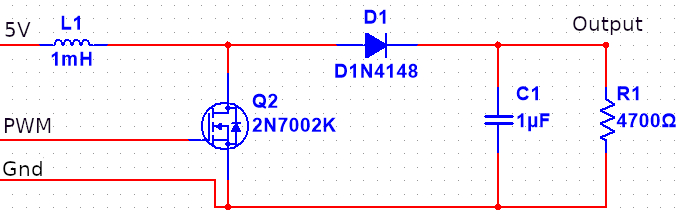
\includegraphics[width=\linewidth]{CircuitDesign.jpg}
    \caption{Multisim diagram of the circuit used in this report}
    \label{fig:pcb}
\end{figure}

